%-------------------------------------------------------------------------------
% Preamble
%-------------------------------------------------------------------------------

\documentclass{article}


%Packages
\usepackage{
	siunitx, % units
  graphicx, % for images
	natbib,
	booktabs
}
\usepackage[letterpaper]{geometry}
\renewcommand{\thefigure}{S\arabic{figure}}
\renewcommand{\thetable}{S\arabic{table}}
\usepackage[breaklinks=true,hidelinks]{hyperref}
\graphicspath{{../../figs/}{./}}

%-------------------------------------------------------------------------------
% Title and Authors
%-------------------------------------------------------------------------------

\title{Supplemental Information for\\``Heavy rainfall in Paraguay during the 2015-2016 austral summer: causes and subseasonal-to-seasonal predictive skill''}
\author{James Doss-Gollin\and \'{A}ngel G. Mu\~{n}oz  \and Simon J. Mason \and Max Past\'{e}n }
\date{\today}

\begin{document}

%% Necessary!
\maketitle

This document contains several supplemental figures referenced in the main text.
Further supporting information is available in the form of source code at \url{github.com/jdossgollin/PYFloods}.

\listoftables
\listoffigures

\clearpage

\begin{table}
	\centering
	\begin{tabular}{lrr}
		\toprule
		{} &  NDJF 2015-16 &  climatology \\
		WT &               &              \\
		\midrule
		1     &      0.272727 &     0.212849 \\
		2     &      0.231405 &     0.184517 \\
		3     &      0.107438 &     0.156342 \\
		4     &      0.206612 &     0.156189 \\
		5     &      0.132231 &     0.149665 \\
		6     &      0.049587 &     0.140438 \\
		\bottomrule
		\end{tabular}
	\caption{Weather type (WT) occurrence fraction during NDJF 2015-16 and Climatology}
\end{table}

\clearpage

\begin{figure}
	\centering
  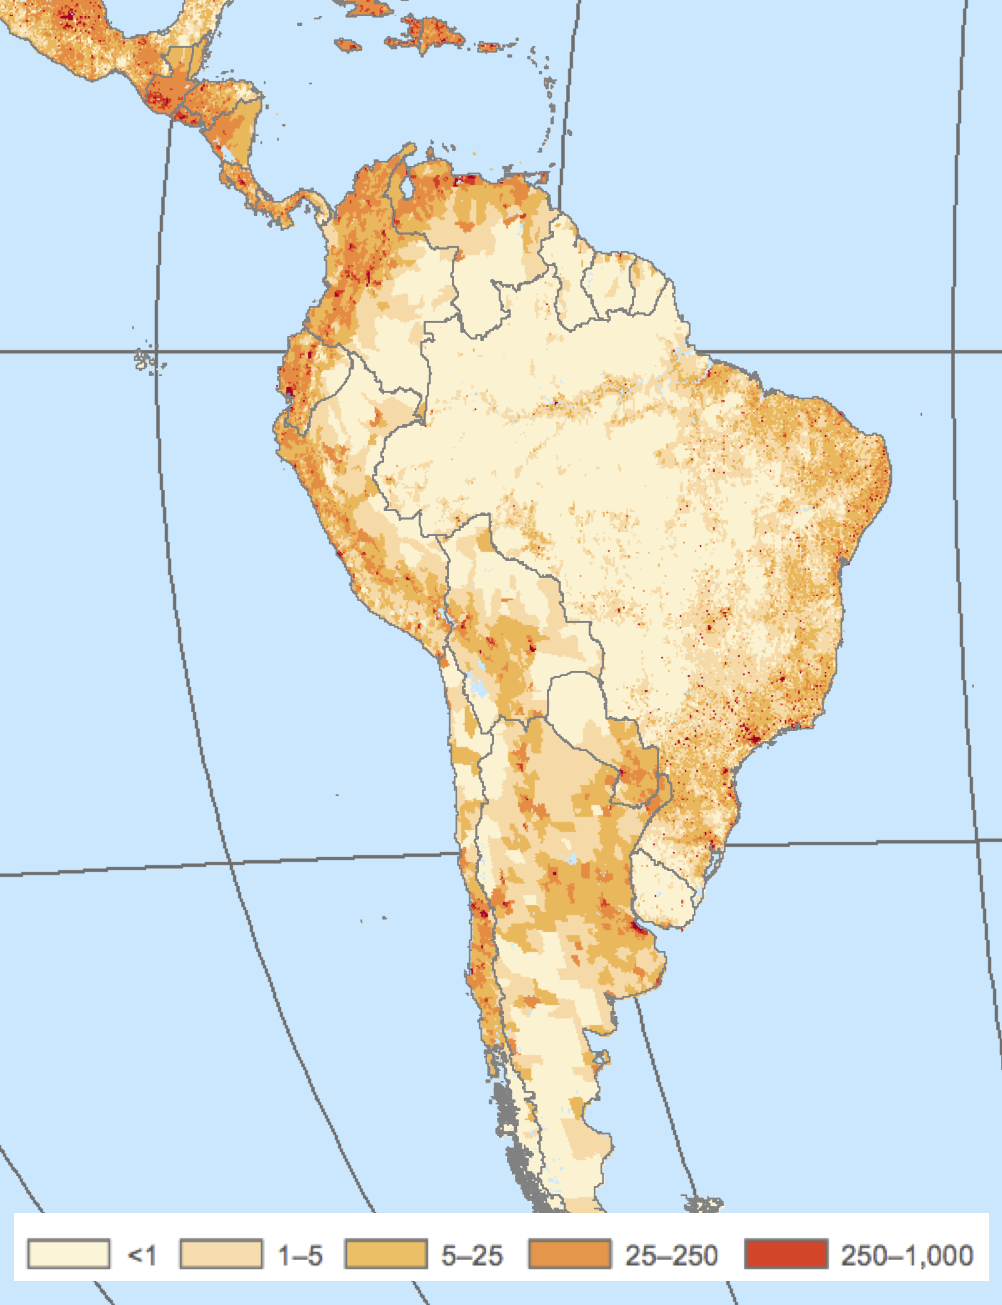
\includegraphics[width=\textwidth,height=0.6\textheight,keepaspectratio=true]{gpw-v4-2015.png}
	\caption{
		Gridded estimate of population density (color; in units of persons per square kilometer) from \citet{GPWv4}.
	}
\end{figure}

\begin{figure}
	\includegraphics[width=\textwidth]{mjo_ts.pdf}
	\caption{
		Time series of MJO evolution during NDJF 2015-16 season.
		$x$-axis shows RMM1 and $y$-axis shows RMM2.
		The associated phases are marked with gray lines and annotated in gray letters.
		The inner circle denotes a ``neutral'' MJO, where the amplitude is less than 1/
		The colored circles describe the time evolution of the system, from 2015-11-01 to 2016-02-29.
		Data from Australian Bureau of Meteorology \citep{Wheeler2004}.
	}
\end{figure}

\begin{figure}
	\includegraphics[width=\textwidth]{nino_34_ts.pdf}
	\caption{
		Monthly NINO 3.4 time series during the study period.
		Each month from November 2015 through February 2016 is specifically marked with a blue dot.
		Data from \citet{Kaplan1998}.
	}
\end{figure}

\begin{figure}
	\includegraphics[width=\textwidth]{nino_sst_anomalies.pdf}
	\caption{
		Monthly SST anomalies during December of several major El Ni\~{n}o events.
		Months shown are (a) December 1982, (b) December 1997, and (c) December 2015.
		Units are in \si{\celsius}.
		Data from \citet{Reynolds2002}.
	}
\end{figure}

\begin{figure}
	\includegraphics[width=\textwidth]{predictors_wtypes.pdf}
	\caption{
		Pearson correlation coefficient between several S2S predictors and weather type occurrence.
		For daily correlation (L), correlations are computed between the binary 0-1 occurrence of each weather type and the predictor.
		Predictors are the 8 MJO phases, encoded as a multinomial variable, and the NINO 3.4 time series, interpolated from monthly to daily values by using the most recent monthly value (no interpolation).
		For monthly correlation (R), correlations are computed between the proportion of occurrence of each weather type and the predictor.
	}
\end{figure}

\begin{figure}
	\includegraphics[width=\textwidth]{wt_classifiability.pdf}
	  \caption{
		  Classifiability index (see Methods) calculated for several chosen values of $K$, representing the number of weather types produced.
		  Results are produced with only 75 simulations for each $K$.
	  }
  \end{figure}

\clearpage
\bibliographystyle{ametsoc2014}
\bibliography{../library}

\end{document}
